\documentclass[10pt, a4paper]{article}
\usepackage{cmap}
\usepackage{amssymb, amsmath}
\usepackage[utf8]{inputenc}
\usepackage{fancyhdr}
\pagestyle{fancy}
\usepackage{listings}
\usepackage{url}
\usepackage{graphicx}
\graphicspath{ {./} }


\setlength{\headheight}{12.4pt}
\setlength{\headsep}{1.5\headheight}

% Übungsblatt-Nummer eintragen
\newcommand{\AssignmentNumber}{1}



\date{} % Kein Datum angegeben
\fancyfoot{} % Seitenzahl unten nicht anzeigen

\lhead{Blatt \AssignmentNumber}

\rhead{Seite \thepage}

\title{Grundlagen der Artificial Intelligence und Logik SS 2021, Übungsblatt \AssignmentNumber}
% TODO Please change group number to correct group
\author{Group BG}
\begin{document}

\newcommand{\seccounter}{\addtocounter{section}{1} \thesection}
\newcommand{\beispiel}[2]{\subsection*{Beispiel #1 \qquad \textnormal{($#2$ P.)}}}
\maketitle
\thispagestyle{fancy}

\newcounter{ale}
\newcommand{\abc}{\item[\alph{ale})]\stepcounter{ale}}
\newenvironment{liste}{\begin{itemize}}{\end{itemize}}
\newcommand{\aliste}{\begin{liste} \setcounter{ale}{1}}
\newcommand{\zliste}{\end{liste}}
\newenvironment{abcliste}{\aliste}{\zliste}

%%%%%%%%%%%%%%%%%%%%%%%%%%%%%%%%%%%%%%%%%%%%%%%%%%%%%%%%%%%%
%  Beispiel 1 - Search approach for Travelling Salesman problem

\beispiel{\seccounter}{1}
Which search approach would you use for solving the “Travelling Salesman Problem (TSP)” within 1 second with 1000 different connection points? Why would you use this approach? 

% TODO Enter the solution for this example here.

To solve the “Traveling Salesman Problem” (TSP) within 1 second for 1000 different nodes, the Local Search method should be used. This is because there are too many possible permutations in the TSP, therefore a Uniformed Search approach would take way longer than 1 second. Local Search is able to find a good solution within this time.


%%%%%%%%%%%%%%%%%%%%%%%%%%%%%%%%%%%%%%%%%%%%%%%%%%%%%%%%%%%%
%  Beispiel 2 - CSP 

\beispiel{\seccounter}{2}
Given the Constraint Satisfaction Problem $x1[1..3], x2[1..3], c1:x1>x2, c2:x2=2.$ Exemplify solution search on the basis of backtracking and forward checking. 


% TODO Enter the solution for this example here.
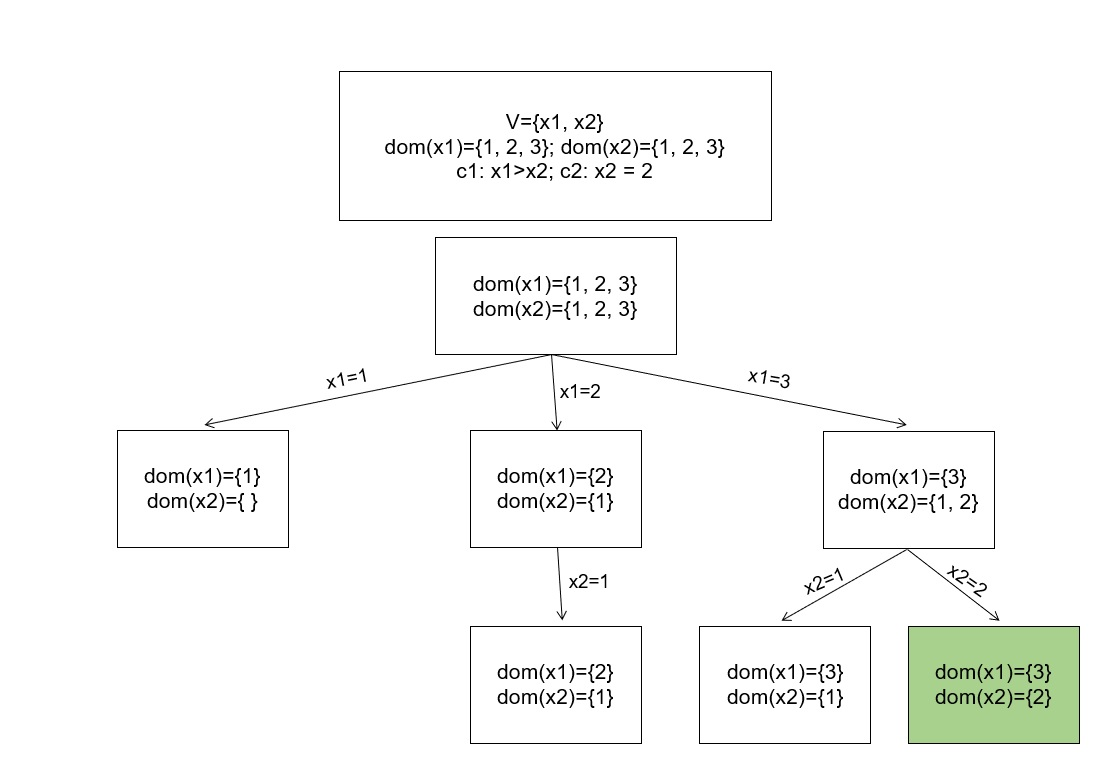
\includegraphics[scale = 0.5]{taskb.jpg}


%%%%%%%%%%%%%%%%%%%%%%%%%%%%%%%%%%%%%%%%%%%%%%%%%%%%%%%%%%%%
%  Beispiel 3 - MiniZinc example 1

\beispiel{\seccounter}{2}
Implement the configuration knowledge base of slide \#18 (slide set on “Constraint Satisfaction”) in MiniZinc.


% TODO Enter the solution for this example here.



%%%%%%%%%%%%%%%%%%%%%%%%%%%%%%%%%%%%%%%%%%%%%%%%%%%%%%%%%%%%
%  Beispiel 4 - MiniZinc example 2

\beispiel{\seccounter}{6}
Implement the TSP in MiniZinc for 10 connection points denoted as {cp1, cp2, .., cp10}. Assure that cp2 is always the first point (of the round trip) and cp5 follows cp3 in each solution.


% TODO Enter the solution for this example here.

%%%%%%%%%%%%%%%%%%%%%%%%%%%%%%%%%%%%%%%%%%%%%%%%%%%%%%%%%%%%
%  Beispiel 5 - Genetic Algorithm

\beispiel{\seccounter}{9}
Implement a solution search for the configuration knowledge base of slide \#18 (see above) on the basis of a genetic algorithm.


% TODO Enter the solution for this example here.
\pagebreak

\end{document} 
